\documentclass[10pt]{article}
\usepackage[margin=1in]{geometry}
\twocolumn
\usepackage{stfloats} 
\usepackage{graphicx}
\begin{document}
\author{Daniel Speyer\\dls2192 \and Johan Mena\\jmm2371}
\title{A Recursive Systemic Profiler}

\twocolumn[
\begin{@twocolumnfalse}
\maketitle

\begin{abstract}
The first task in writing any performant code is to understand where it is spending its time. This allows you both to apply optimizations where they will make a difference, and to not optimize where it won’t make a difference. The standard tools for this are profilers, which measure where the process spends its time while running. However many processes spend most of their total wall time in actions not measured by traditional profilers. Here, we propose a system that can give a more complete view of the causes of an application’s performance.
\end{abstract}

\end{@twocolumnfalse}
]

\section{Introduction}
 Lorem ipsum dolor sit amet, consectetur adipiscing elit. Maecenas malesuada, libero tempus congue tempus, velit sem ultricies enim, quis pretium odio turpis nec nulla. Aliquam mollis magna in est semper fermentum. Suspendisse sed orci ullamcorper, hendrerit neque quis, lacinia dui. Quisque id enim at libero consectetur hendrerit. Nam enim nunc, bibendum in vulputate in, dictum vitae risus. Proin molestie arcu tortor, ac cursus erat commodo vitae. Integer sodales erat et magna porttitor ultrices. Nulla facilisi. Quisque quam eros, convallis eu nunc porttitor, imperdiet convallis lorem. Quisque scelerisque egestas tincidunt. Vivamus pharetra ex ligula, ac aliquam mauris dapibus quis. Cras non ligula eu ante mollis malesuada. Nam est lacus, fringilla nec mi eget, iaculis aliquet nisi.

In hac habitasse platea dictumst. Suspendisse potenti. Nullam vitae dolor consectetur, sollicitudin ex at, suscipit leo. Suspendisse sit amet mauris auctor orci condimentum aliquet tristique ac arcu. Nam sollicitudin mauris vel quam vulputate, id scelerisque arcu bibendum. Pellentesque vitae urna sed enim dignissim pulvinar in et eros. Mauris nec risus dapibus, ultricies est et, malesuada mauris. Suspendisse potenti. Sed quis tellus eu velit facilisis viverra aliquam nec ante.

\section{Background: Tools to Get Data}

\subsection{Linux Perf Events}

\subsection{Dtrace}

\section{Other Visualizations}

\subsection{flamegraphs}

\section{Recursive Systemic Profiler}

\subsection{Concepts}

\subsubsection{Pseudostacks and Critical Pathes}

\subsection{Views}

\subsubsection{Process Running View}

\begin{figure}[h]
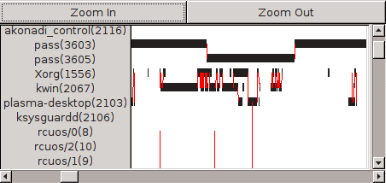
\includegraphics[width=3.25in]{screenshot}
\caption{The Process Running View}
\end{figure}

\subsection{Implementation}
\subsubsection{Data Collection}
\subsubsection{Assembling Runs, Sleeps and Links}
\subsubsection{Algorithms For Link Finding}
\subsubsection{Working Around Interrupts}
\subsubsection{Recursive Stack Making}
\subsubsection{Assembling Pseudostacks}
\subsubsection{Consolidating}
\subsubsection{Visualizing}
\section{Evalutation}
\subsection{apt-get}
\subsubsection{Visualization}
\subsubsection{How Much Is Explained}
\subsubsection{Comparisons}
\subsection{Other tests}
\subsubsection{squirrelmail}
\subsubsection{chrome load}
\end{document}
